\documentclass{beamer}
%TODO:
%warum müssen wir supersingular curves benutzen?
%j-invariants
% wozu brauchen wir ramanujan graphs?

% Choose how your presentation looks.
%
% For more themes, color themes and font themes, see:
% http://deic.uab.es/~iblanes/beamer_gallery/index_by_theme.html
%
\mode<presentation>
{
  \usetheme{boxes}      % or try Darmstadt, Madrid, Warsaw, AISEC ...
  \usecolortheme{dolphin} % or try albatross, beaver, crane, ...
  \usefonttheme{default}  % or try serif, structurebold, ...
  \setbeamertemplate{navigation symbols}{}
  \setbeamertemplate{caption}[numbered]
} 

%\usepackage{fhgfont} funktioniert leider noch nicht
\usepackage[shortlabels]{enumitem} % counter styles for enumerations
\usepackage[font=footnotesize]{caption} %for attributing pictures
\usepackage[english]{babel}
\usepackage[utf8x]{inputenc}
\usepackage{braket} % dirac notation
\usepackage{amsmath} % math symbols
\usepackage{amssymb} % other symbols
\graphicspath{ {img/} }
\usepackage{svg} %insert svg
\usepackage{svg-extract} %insert svg
\usepackage{graphicx} % insert pdfs
\newenvironment{rcases} % for right braces
{\left.\begin{aligned}}
	{\end{aligned}\right\rbrace}

\title[SIKE]{SIKE - Supersingular Isogeny Key Encapsulation}
\author{Jonas von der Heyden}
\institute{FU Berlin}
\date{4.6.19}

\begin{document}
\newcommand{\source}[1]{\caption*{Source: {#1}} } %for attributing pictures
\begin{frame}
  \titlepage
\end{frame}

% Uncomment these lines for an automatically generated outline.
\begin{frame}{Outline}
  \tableofcontents
\end{frame}

\section{Introduction}

\begin{frame}{Introduction}

	\begin{itemize}
  		\item Goal of this presentation: Give a high-level overview of SIKE protocol
  		% advantages: small key sizes, no shor's algorithm because no group action
  		%disadvantage: too slow (but still in early stages)
	\end{itemize}

\end{frame}
\begin{frame}{Comparison of DH, ECDH and SIDH}
\begin{figure} %TODO: DH an Tafel
	\centering
	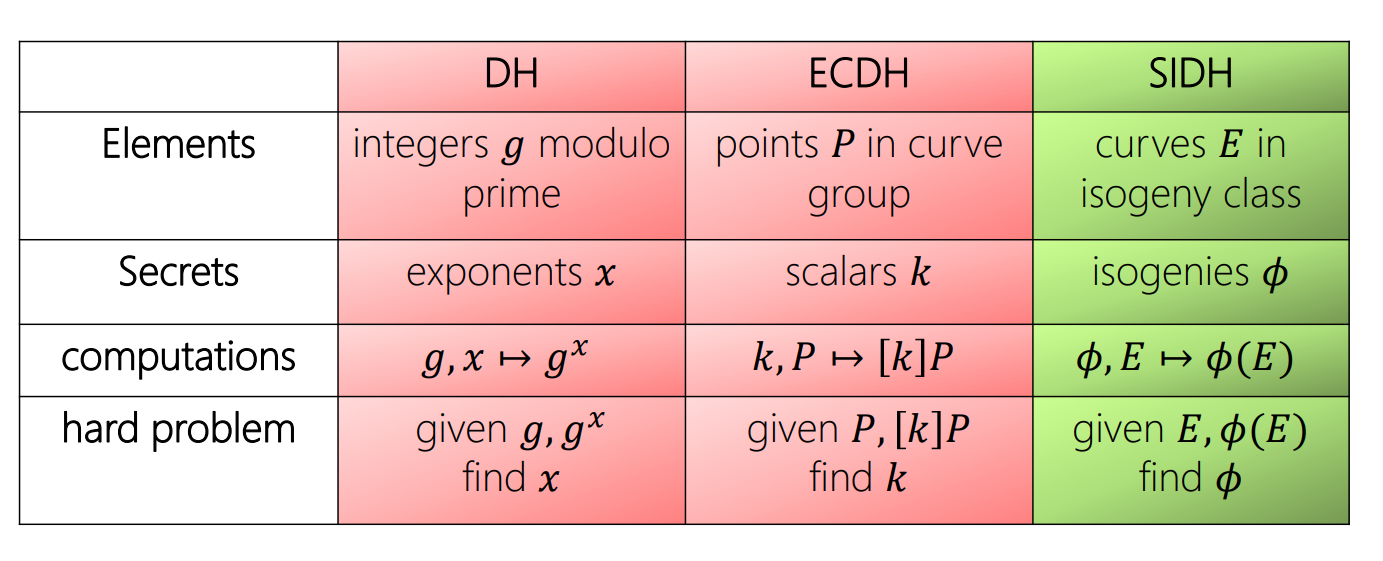
\includegraphics[width=1\linewidth]{dh_ec_iso}
	\label{fig:dh_ec_iso}
\end{figure}
\end{frame}



\section{Mathematical primitive}

\subsection{Elliptic Curves}

\begin{frame}{Elliptic curves}
	Which of the figures is \textit{not} an elliptic curve?
	\begin{figure}
		\begin{minipage}{0.48\textwidth}
			\centering
			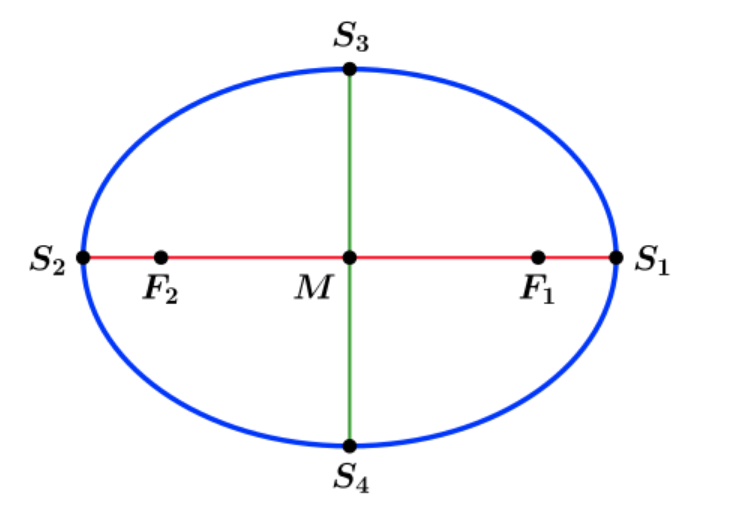
\includegraphics[width=.7\linewidth]{ellipse}
			\label{fig:ellipse}
		\end{minipage}\hfill
		\begin{minipage}{0.48\textwidth}
			\centering
			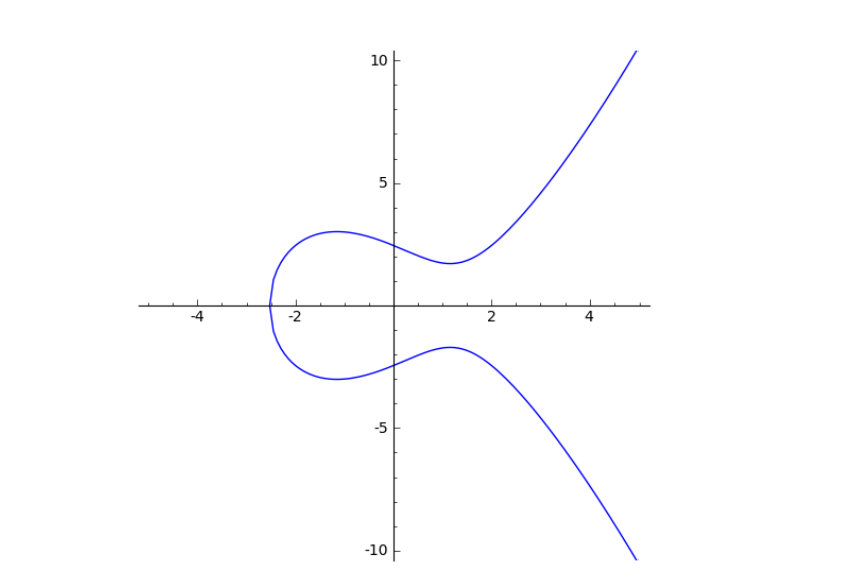
\includegraphics[width=.7\linewidth]{elliptic_curve}
			\label{fig:elliptic_curve}
		\end{minipage}
	\end{figure}
	\begin{figure}
	\begin{minipage}{0.48\textwidth}
		\centering
		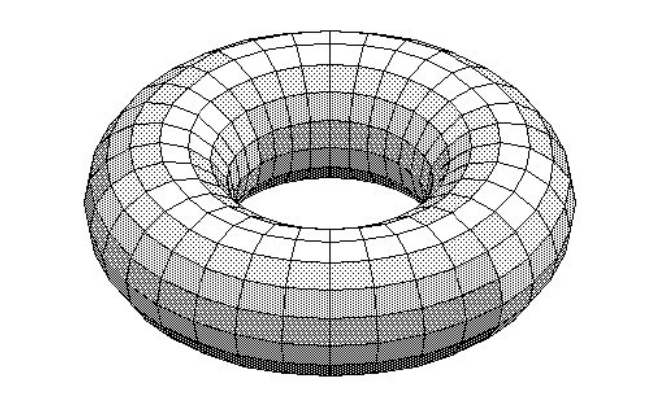
\includegraphics[width=.7\linewidth]{elliptic_curve_c}
		\label{fig:elliptic_curve_c}
	\end{minipage}\hfill
	\begin{minipage}{0.48\textwidth}
		\centering
		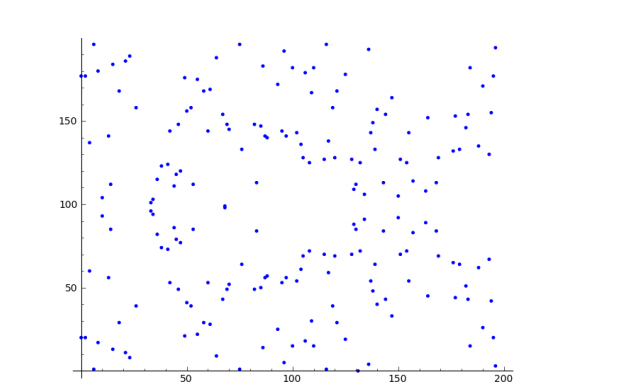
\includegraphics[width=.7\linewidth]{elliptic_curve_fp}
		\label{fig:elliptic_curve_fp]}
	\end{minipage}
\end{figure}


	% image of ellipse
\end{frame}

\begin{frame}{Elliptic curves}
	Which of the figures is \textit{not} an elliptic curve?
\begin{figure}
	\begin{minipage}{0.48\textwidth}
		\centering
		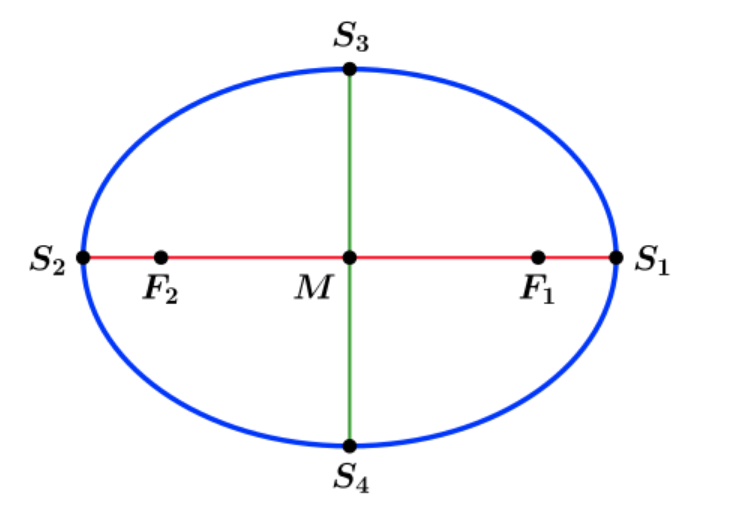
\includegraphics[width=.7\linewidth]{ellipse}
		\caption{Ellipse}\label{fig:ellipse}
	\end{minipage}\hfill
	\begin{minipage}{0.48\textwidth}
		\centering
		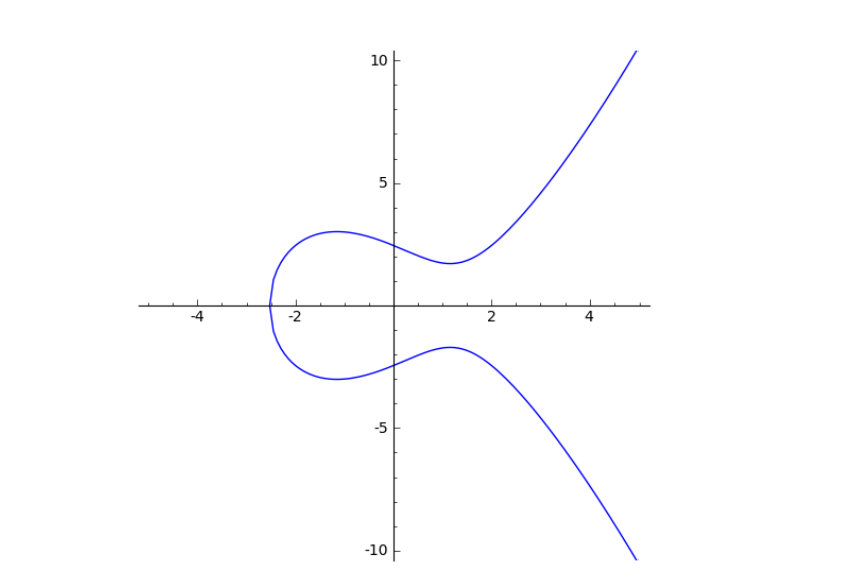
\includegraphics[width=.7\linewidth]{elliptic_curve}
		\caption{Elliptic Curve over $\mathbb{R}$}\label{fig:elliptic_curve}
	\end{minipage}
\end{figure}
\begin{figure}
	\begin{minipage}{0.48\textwidth}
		\centering
		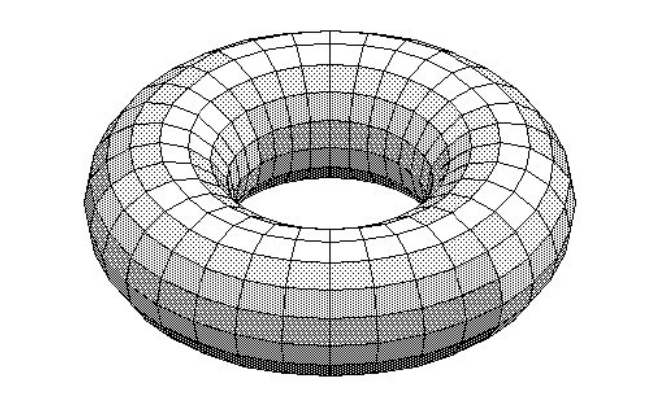
\includegraphics[width=.7\linewidth]{elliptic_curve_c}
		\caption{Elliptic Curve over $\mathbb{C}$}\label{fig:elliptic_curve_c}
	\end{minipage}\hfill
	\begin{minipage}{0.48\textwidth}
		\centering
		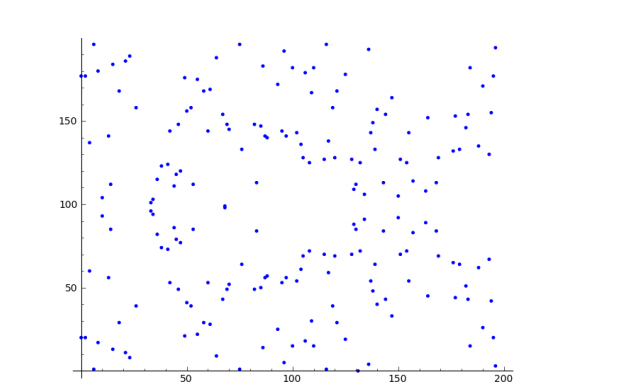
\includegraphics[width=.7\linewidth]{elliptic_curve_fp}
		\caption{Elliptic Curve over $\mathbb{F}_p$}\label{fig:elliptic_curve_fp]}
	\end{minipage}
\end{figure}

\end{frame}
\begin{frame}{Elliptic curves}
What is an elliptic curve?
\begin{itemize}[\textbullet]
	\item Historically, elliptic curves were used to calculate the circumference of an ellipse
	\item An elliptic curve is the set of solutions to a \textit{Weierstrass equation} of the form $Y^2=X^3+AX+B$
\end{itemize}

\begin{figure}
	\centering
	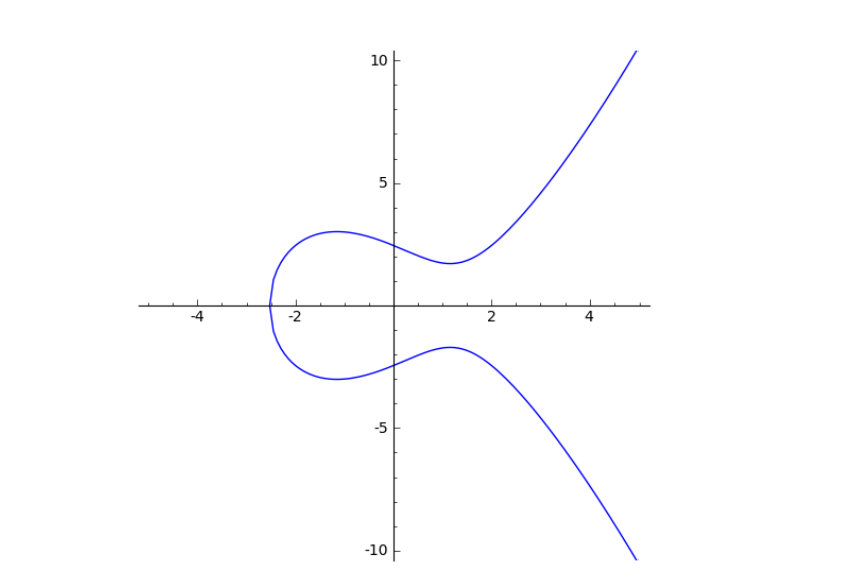
\includegraphics[width=.7\linewidth]{elliptic_curve}
	\label{fig:elliptic_curve}
\end{figure}
	
\end{frame}

\begin{frame}{Abelian Groups (G,+) over Elliptic Curves}
\begin{figure}
	\begin{minipage}{0.5\textwidth}
		\centering
		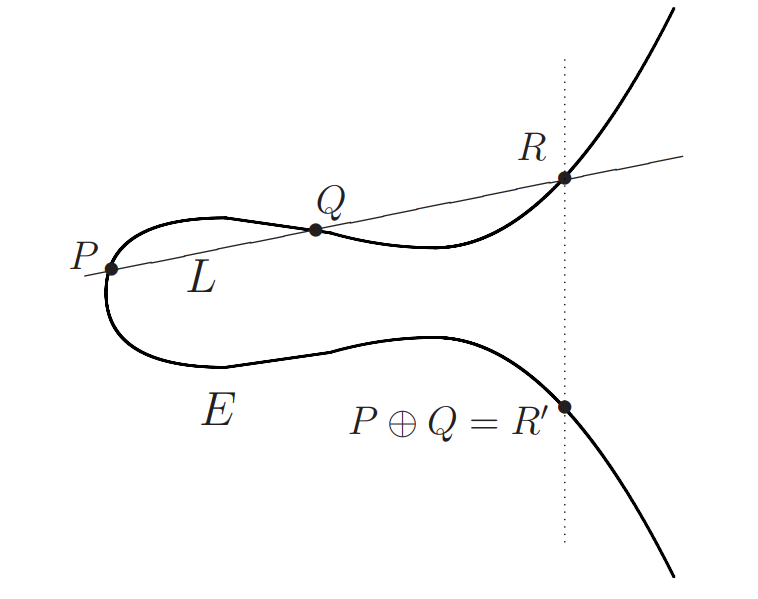
\includegraphics[width=1\linewidth]{P+Q}
		\caption{P+Q}\label{fig:p+q}
	\end{minipage}\hfill
	\begin{minipage}{0.48\textwidth}
		\centering
		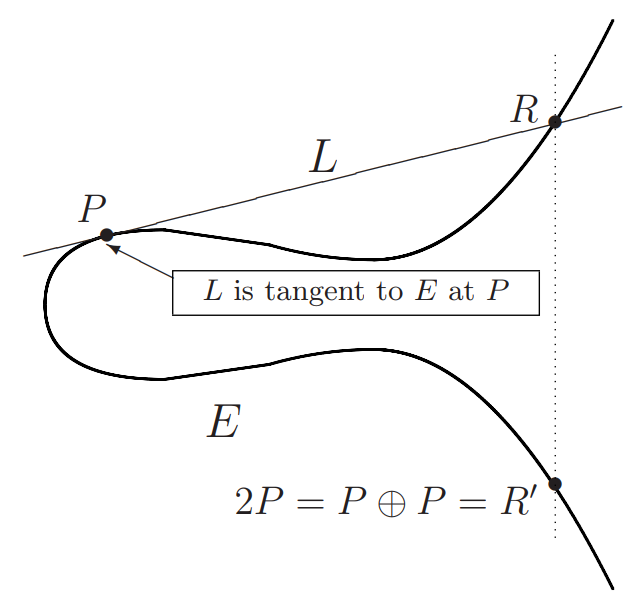
\includegraphics[width=1\linewidth]{P+P}
		\caption{P+P}\label{fig:p+p}
	\end{minipage}
\end{figure}

\end{frame}
\begin{frame}{Abelian Groups (G,+) over Elliptic Curves}
\begin{figure}

		\centering
		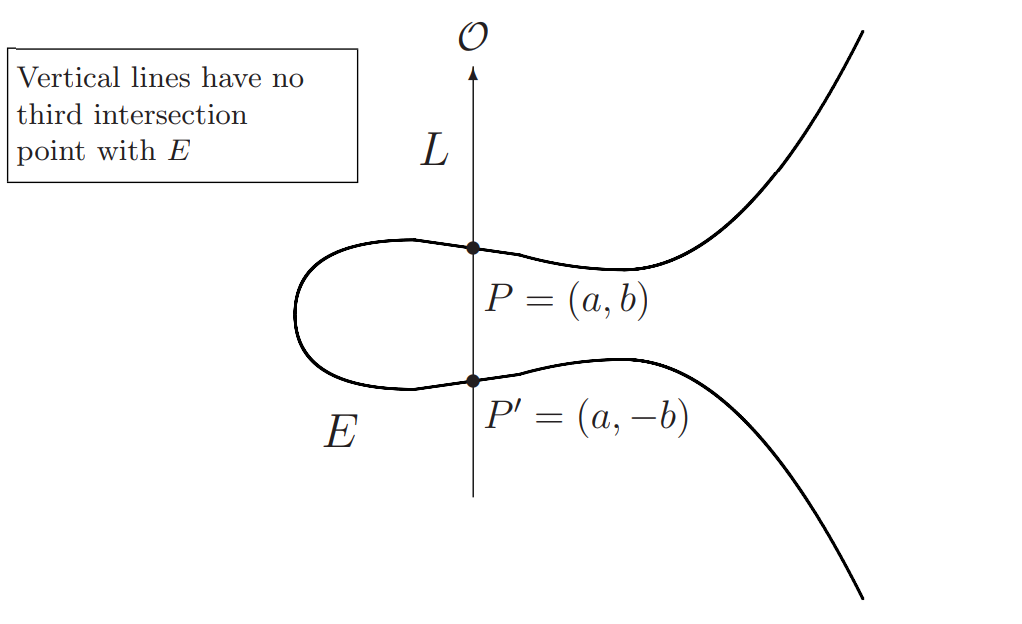
\includegraphics[width=1\linewidth]{P-P}
		\caption{P-P}\label{fig:p-p}


\end{figure}
\end{frame}
\begin{frame}{Abelian Groups (G,+) over Elliptic Curves}
	Let E be an elliptic curve. Then the addition law on E has the following properties:
	\begin{enumerate}[1.]
		\item $P + \mathcal{O} = \mathcal{O} + P$ (Identity)
		\item $P + (-P) = \mathcal{O}$ (Inverse)
		\item $(P + Q) + R = P + (Q + R) $ (Associative)
		\item $P + Q = Q + P$ (Commutative)
	\end{enumerate}

\end{frame}

\begin{frame}{Elliptic Curve addition algorithm}
	Let $E : Y^2 = X^3 + AX + B$ be an elliptic curve and let $P_1$ and $P_2$ be points on E.
	\begin{enumerate}[1.]
		\item If $P_1 = \mathcal{O}$, then $P_1 + P_2 = P_2$\pause
		\item Otherwise, if $P_2=\mathcal{O}$, then $P_1 + P_2 = P_1$\pause
		\item Otherwise, write $P_1 = (x_1,y_1)$ and $P_1 = (x_2,y_2)$\pause
		\item If $x_1 = x_2$ and $y_1=-y_2$, then $P_1+P_2=\mathcal{O}$\pause
		\item Otherwise, define \\
		\qquad \qquad \qquad$\lambda =
		\begin{cases}
			\frac{y_2-y_1}{x_2-x_1}\text{\quad if }P_1 \neq P_2\\\pause
			\\
			\frac{3x_1^2 +A}{2y_1}\text{\quad if }P_1=P_2 \pause
		\end{cases}$\\
		\vspace{5mm}
		and let $x_3=\lambda^2-x_1-x_2$  \hfill and $y_3=\lambda(x_1-x_3)-y_1$.\\
		\vfill
		Then $P_1+P_2=(x_3,y_3)$.
	\end{enumerate}
\end{frame}


\begin{frame}{Elliptic Curves over finite fields}
	\begin{itemize}[\textbullet]
		\item An elliptic curve over $\mathbb{F}_p$ is an equation of the form $E:Y^2=X^3+AX+B$
		\item The set of points of E with coordinates in $\mathbb{F}_p$ is the set $E(\mathbb{F}_p)=\{(x,y):x,y\in \mathbb{F}_p$ satisfy $y^2=x^3+Ax+B \} \cup \{\mathcal{O}\}$
		\item Elliptic curve addition algorithm continues to work in $E(\mathbb{F}_p)$
		\item Addition law continues to satisfy properties of Abelian Groups
		\item If \#X is the cardinality of a set X, then \#$E(\mathbb{F}_q) = q+1-t$ for $|t|\leq 2\sqrt{q}$
		\item An elliptic curve $E(\mathbb{F}_q)$ is called \textit{supersingular} if $p \mid t$ where $q=p^a$
		\item It follows for all supersingular curves: $\#E(\mathbb{F}_q^n)\equiv 1 \bmod p$ for all $n\in \mathbb{N}$ and $p>3$
	\end{itemize}
	%TODO: (1)Beispiel!, (2) Konsequenz aus letztem Punkt
	
\end{frame}

\begin{frame}{ECDLP}
\end{frame}

\subsection{Points of finite order} 

\begin{frame}{Points of finite order}
\begin{itemize}[\textbullet]
	\item A point $P\in E$ satisfying $mP=\mathcal{O}$ is called a point of order m in the group E
	\item $E[m] = \{P\in E: mP = \mathcal{O}\}$ is also called the m-torsion group of E and includes all points of order $m$ in $E$
	\item $E[m] $ is a subgroup of E since if $P,Q\in E[m]$ then also $P+Q$ and $-P$
\end{itemize}
 	
\end{frame}

\subsection{Isogenies}
\begin{frame}{Group homomorphisms}
Properties of group homomorphisms:
\begin{itemize}[\textbullet]
	\item Given 2 groups (G,+), (H,$\oplus$) a group homomorphism is a function $\phi: G \to H$ such that $\phi(u + v) = \phi(u) \oplus \phi(v)$ 
	\item $\phi(e_G) = e_H$ where $e_G$ and $e_H$ are the identity elements of G and H
	\item The kernel of $\phi$ is the set of elements in $G$ which are mapped to the identity in $H$:
	$ker(\phi) \equiv \{u\in G:\phi(u)=e_H\}$
\end{itemize}
	 
	
	%Schaubild an Tafel
	\begin{block}{Example}
		$\phi: \mathbb{Z}\to\mathbb{Z}/3\mathbb{Z}$ is surjective and it's kernel consists of all elements in $\mathbb{Z}$ divisible by 3
		
		
	\end{block}
\end{frame}
\begin{frame}{Types of Homorphisms}
	\begin{itemize}[\textbullet]
		\item Isomorphism: A group homomorphism that is bijective % Schaubild Graphisomorphie
		\item Endomorphism: A group homomorphism $\phi: G \to G$
		\item Isogeny: A group homomorphism $\phi : G \to H$ with a finite kernel
	\end{itemize}

\begin{block}{Isogeny Example}
	Multiplication map $[n]: E \to E$ defined by $[n]P = P + P + ...+ P$ ($n$ times):
	\begin{itemize}[\textbullet]
		\item Maps 0 to itself and is surjective
		\item $ker[n] = E[n]$, therefore kernel is finite (if elliptic curve is defined over $\mathbb{F}_p$)
		\item Isogeny [n] can be calculated with elliptic curve addition algorithm %Beispiel an Tafel?
		
	\end{itemize}
%	Any 2 elliptic curves $E_1,E_2$ over $\mathbb{F}_q$ are isogenous iff $\#E_1(\mathbb{F}_q) = \#E_2(\mathbb{F}_q)$ ($E_1$ and $E_2$ have the same number of points). What about the kernel?
\end{block}

\end{frame}

\begin{frame}{Isogenies of elliptic curves}  %TODO: Example 3 aus Galbraith an Tafel
Let $E_1,E_2$ be 2 elliptic curves over $\mathbb{F}_q$. Then an isogeny is a morphism $\phi: E_1 \to E_2$ s.t.:
\begin{itemize}[\textbullet]
	\item $\phi(0_{E_1})= 0_{E_2}$
	\item $\#E_1(\mathbb{F}_q) = \#E_2(\mathbb{F}_q)$
	\item there exists a dual isogeny $\hat{\phi}: E_2 \to E_1$
	\item up to isomorphism it is uniquely defined by it's kernel $ker(\phi)$. Because a kernel is also a finite subgroup G of $E_1$ we can also say that $E_2$ is $E_1/G$
	\item equivalently it is also uniquely defined up to isomorphism by it's j-invariant $j(E)=1728\frac{4A^3}{4A^3+27B^2}$
	%TODO: how does j-invariant work?
\end{itemize}


\end{frame}



\section{Cryptosystem}

\subsection{SIDH protocol}

\begin{frame}{The SIDH protocol: Main idea}
Idea: Create Diffie-Hellman exchange over isogenies of elliptic curves. %DLDH an Tafel zeichnen
\begin{figure}
	\begin{minipage}{0.5\textwidth}
		\centering
		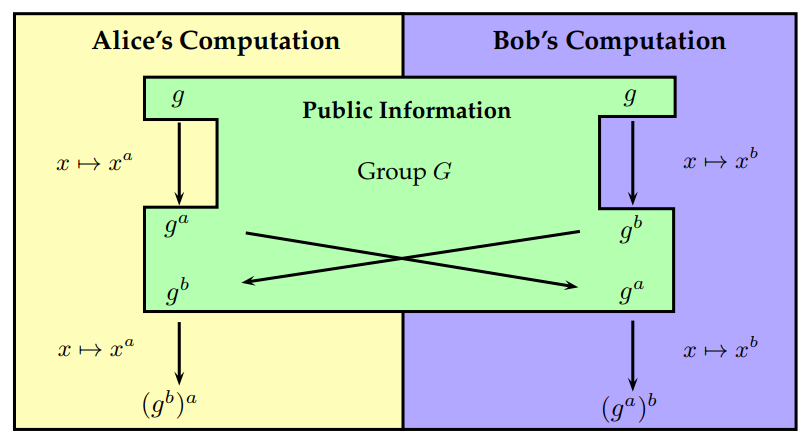
\includegraphics[width=1\linewidth]{DLDH}
		\caption{Discrete Logarithm Diffie-Hellman}\label{fig:dldh}
	\end{minipage}\hfill
	\begin{minipage}{0.48\textwidth}
		\centering
		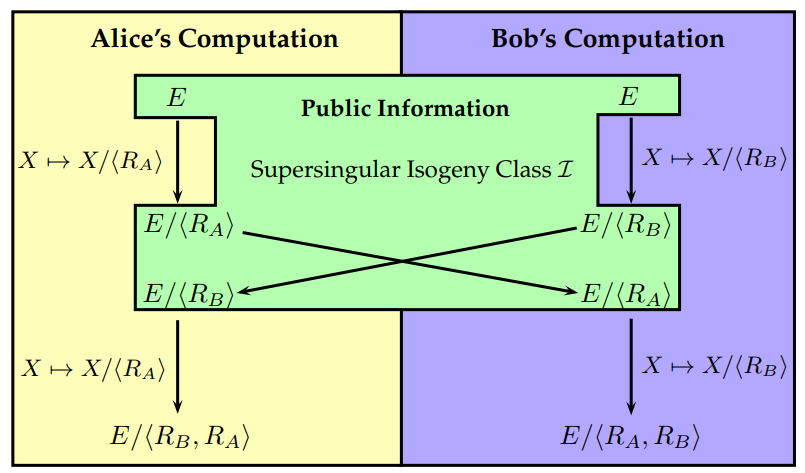
\includegraphics[width=1\linewidth]{SIDH}
		\caption{Supersingular Isogeny Diffie-Hellman}\label{fig:sidh}
	\end{minipage}
\end{figure}

\end{frame}


\begin{frame}{The SIDH protocol: Setting up parameters}
\begin{enumerate}[1.]
	\item Generate public parameters:
	\begin{enumerate}[(a)]
		\item Choose $2^{e_A},3^{e_B}$, search for a prime $p=2^{e_A}3^{e_B}f\pm 1$ %and compute $q=p^2$
		\item Set $q=p^2$ and construct elliptic curve $E$ over $\mathbb{F}_q$ of cardinality $(2^{e_A}3^{e_B}f)^2$ %wie geht das?
		\item Find bases $P_A,Q_A$ and $P_B,Q_B$ s.t. $\langle P_A,Q_A\rangle$ = $E[2^{e_A}]$ and $\langle P_B,Q_B\rangle$ = $E[3^{e_B}]$ %TODO: wie schwierig ist das?
	\end{enumerate}
	\item Generate secret parameters:
	\begin{enumerate}[(a)]
		\item Alice picks 2 random secret elements $m_A,n_A < 2^{e_A}$, Bob picks 2 random secret elements $m_B,n_B < 2^{e_B}$
		\item Alice computes secret isogeny $\phi_A : E \to E/A$ with kernel $\langle [m_A]P_A+[n_A]Q_A\rangle$, Bob computes secret isogeny $\phi_B : E \to E/B$ with kernel $\langle [m_B]P_B+[n_B]Q_B\rangle$
	\end{enumerate}

\end{enumerate}
\end{frame}

\begin{frame}{The SIDH protocol: Commutative Action}

\begin{enumerate}[1.]
	\item Compute $\phi_A^{\prime},\phi_B^{\prime}$

	\begin{enumerate}[(a)]
		\item Alice computes the image $\{\phi_A(P_B),\phi_A(Q_B)\} \subset E/A$ and sends it to Bob and vice versa
		\item Now Alice is able to compute the point $T_A=[m_A]\phi_B(P_A) + [n_A]\phi_B(Q_A)$ in $E/B$
		\item Next Alice computes the isogeny $\phi_A^{\prime}$ with kernel $\langle T_A \rangle$ to the curve $E/AB$
		\item Bob proceeds \textit{mutatis mutandis}. On the next slide we will show that $\langle T_B \rangle  = ker(\phi_B^{\prime})=ker(\phi_A^{\prime})=\langle T_A \rangle$ and therefore $E/AB \simeq E/BA$.
	\end{enumerate}
	\item Alice and Bob compute the j-invariant $j(E/AB)=j(E/BA)$ to form a shared secret key 
\end{enumerate}
\end{frame}

\begin{frame}{The SIDH protocol: Correctness}
\textbf{Question:} Why is $ker(\phi_B^{\prime})=ker(\phi_A^{\prime})$?\\
\vspace{5mm}
\textbf{Lemma 1:} Let $\phi_1: G_1 \to G_2$ and $\phi_2: G_2 \to G_3$ be group homomorphisms with $ker(\phi_1) = \langle K_1 \rangle$ and $ker(\phi_2) = \phi_1(\langle K_2 \rangle)$. Then for $\phi:G_1 \to G_3$ defined by $\phi=\phi_2 \circ \phi_1$ we have $ker(\phi) =\langle K_1,K_2\rangle$.\\ %beweis an Tafel
\vspace{5mm}

\textbf{Theorem 2:} $ker(\phi_B^{\prime} \circ \phi_A) = ker(\phi_A^{\prime} \circ \phi_B)$\\
\textbf{Proof:}
	\begin{enumerate}[(i)]
		\item $ker(\phi_B^{\prime})=\phi_A(\langle [m_B]P_B + [n_B]Q_B)\rangle)$
		\item $ker(\phi_A)=\langle [m_A]P_A + [n_A]Q_A\rangle$
		\item $ker(\phi_B^{\prime} \circ \phi_A) \stackrel{\text{Lemma 1}}{=} \langle [m_A]P_A + [n_A]Q_A, [m_B]P_B + [n_B]Q_B \rangle$
		\item The application of Lemma 1 on $\phi_A^{\prime} \circ \phi_B$ yields the same kernel
	\end{enumerate}

\vfill

Since isogenies are uniquely defined by their kernel, $E/AB \simeq E/BA$.

\end{frame}

\begin{frame}{The SIDH protocol: Visualization} %besser an due Tafel malen!
\begin{figure}
	\centering
	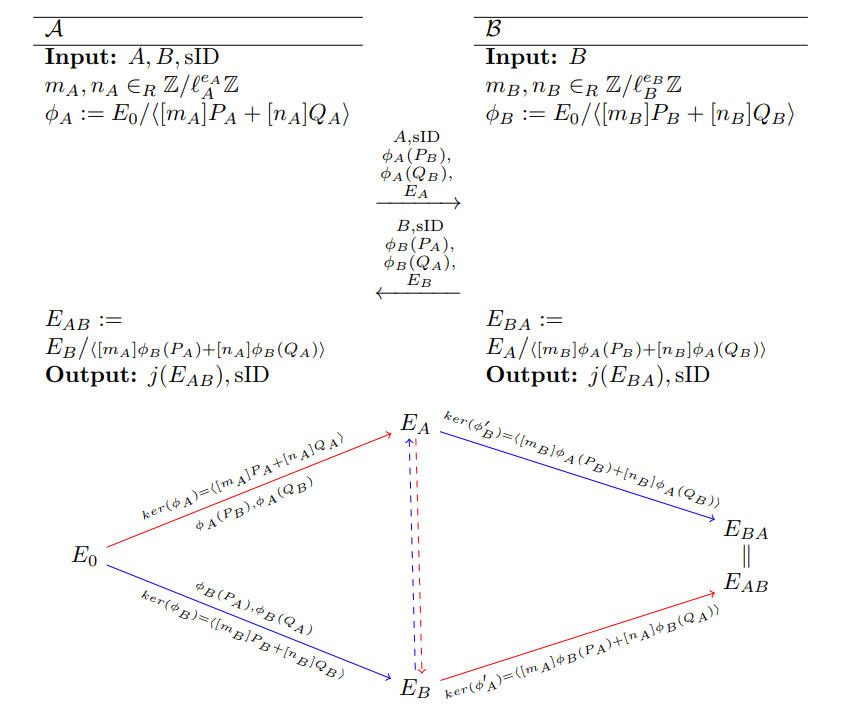
\includegraphics[width=0.7\linewidth]{SIDH_big}
	\caption{SIDH}
	\label{fig:sidh_big}
\end{figure}
\end{frame}

\begin{frame}{The SIKE protocol}

How does the SIKE specification for NIST PQ competition differ from SIDH?

\begin{itemize}[\textbullet]
%	\item SIKE is a key encapsulation scheme that uses the SIDH protocol to generate a shared key between 2 parties % TODO: vielleicht key encapsulation kurz zeigen
	\item SIKE is IND-CPA-secure and IND-CCA-secure %TODO: noch herausfinden warum
	\item SIKE uses compression to reduce key sizes and computes private keys in constant time to defend against side-channel attacks
\end{itemize}

\end{frame}

\subsection{Computation Details and Efficiency}

\begin{frame}{Efficiently computing isogenies}


	\textbf{Problem:} Computing $\phi_G : E \to E/A$ from $E$ and $A$ takes time polynomial in $\#A$. Since $2^{e_A} \in \mathcal{O}(\sqrt{p})$, this is not acceptable.\\
	\vfill
	\textbf{Solution:} Compute isogeny of large degree as a composition of isogenies of small degree. Then $\phi = \phi_1 \circ \dots \circ \phi_k \circ [n]$ where $\phi_1 \circ \dots \circ \phi_k$ are isogenies of prime degree that are defined over $\mathbb{F}_q$ and $deg(\phi) = n^2 \prod^k_{i=1} deg(\phi_i)$.\\
	 While computing the composition of $t$ isogenies of degree $t$ takes time proportional to $t$, the cost of computing the composition in a single step is in $\mathcal{O}(2^t)$ 

\end{frame}

\section{Areas of use}

\begin{frame}{Areas of use}
SIKE is characterized by having a very small key size but being fairly inefficient in the key-generation. Therefore it seems to be most suitable for:
\begin{itemize}[\textbullet]
	
	\item Securing applications where bandwidth is a more precious commodity than computational cycles, e.g. Bitcoin and Tor
	\item Securing TLS once further research has resulted in better performance
	\item Use in a hybrid cryptosystem combining untested post-quantum-cryptography with a conventional encryption scheme since it can use the same elliptic curve like ECDH	
\end{itemize}
At this stage, it is not suitable for use in embedded devices or microcontrollers due to high energy demand.
\end{frame}

\section{Security \& Complexity}

% SIKE spec 4.1
% perfect forward secrecy
% reuse of keys
% sidh security paper p.5
% side channel & error attacks?
% galbraith: security of all schemes of this type depends on the difficulty of computing the endomorphism ring of a supersingular elliptic curve
%why supersingular: because of endomorphism ring
\begin{frame}{Security assumptions} %Mündlich: Es wird angenommen, dass diese Probleme schwer sind.
\begin{enumerate}[1.]
	\item \textbf{Computational Supersingular Isogeny problem:}\\
	Let $\phi_A:E\to E/A$ be an isogeny with $ker(\phi_A)=\langle [m_A]P_A+[n_A]Q_A\rangle$. Given $E/A$ and the values $\phi_A(P_B),\phi_A(Q_B)$ find a generator $R_A$ of $\langle [m_A]P_A+[n_A]Q_A\rangle$\pause
	\vspace{5mm}
	\item \textbf{Computational Supersingular Diffie-Hellman problem:}\\ 
	Let $\phi_A:E\to E/A$ be an isogeny with $ker(\phi_A)=\langle [m_A]P_A+[n_A]Q_A\rangle$ and let $\phi_B:E\to E/A$ be an isogeny with $ker(\phi_B)=\langle [m_B]P_B+[n_B]Q_B\rangle$
	Given $E/A,E/B$ and the points $\phi_A(P_B),\phi_A(Q_B),\phi_B(P_A),\phi_B(Q_A)$ find the j-invariant of $E/\langle [m_A]P_A+[n_A]Q_A,[m_B]P_B+[n_B]Q_B \rangle$\pause
	\vfill
	It is being assumed that both problems are hard. There is no reduction to an NP-complete problem.
\end{enumerate}
\end{frame}

\begin{frame}{Known attacks: claw algorithm}
The best known attack against SIKE is the "claw algorithm":

\begin{enumerate}[(i)]
	\item Given $\phi : E \to E_A$ with $deg(\phi) = 2^{e_A}$, find $\phi$
	\item Start with computing all $2^{e_A/_2}$-isogenies of one curve in $\mathcal{O}(p^{1/4})$ space and time
	\item Then compute all $2^{e_A/_2}$-isogenies of the other curve and look for a collision
	\item Overall space and time requirement is in $\mathcal{O}(p^{1/4})$ on a classical computer and $\mathcal{O}(p^{1/6})$ quantumly
\end{enumerate}
\end{frame}
\begin{frame}{Known attacks: endomorphism ring}


\begin{itemize}[\textbullet]
	\item The endomorphism ring of E is the set of isogenies from E to itself: $End(E) = \{\phi:E\to E\} \cup \{0\}$
	\item Addition of isogenies is defined using elliptic curve addition as $(\phi_1+\phi_2)(P) =  \phi_1(P) + \phi_2(P)$
	\item Multiplication is the composition $\phi_1 \circ \phi_2$
	\item Given $E$ and $End(E)$, computing $\phi: E \to E'$ can be reduced to computing $End(E')$. This is shown to be possible in subexponential time on quantum computers, if E is ordinary
	\item Unlike ordinary curves, the endomorphism ring of supersingular curves is non-commutative and is therefore not susceptible to the quantum attack
\end{itemize}



\end{frame}

\begin{frame}{Resistance against side-channel and fault attacks}
Attack vectors for timing, power and fault analysis:
\begin{itemize}[\textbullet]
	\item Computation of the hidden kernel point
	\item Computation of the secret isogeny
\end{itemize}

\vfill

As a countermeasure all secret values are being computed using constant-time-functions. However, this does not defend against fault injection attacks.


\end{frame}

\begin{frame}{Passive and active security}

SIKE is IND-CPA and IND-CCA secure.

\begin{itemize}[\textbullet]
	\item \textbf{IND-CPA}: SIDH can be modified to be secure against a passive attacker by converting it into an ElGamal scheme
	\item \textbf{IND-CCA}: By using a Key-Encapsulation-Mechanism (KEM) it is possible to prevent any active attacks as well
\end{itemize}

%costello slides
\end{frame}

\section{Discussion}

\begin{frame}{Conclusion}
%Nachteil: sehr kompliziert, daher ist Sicherheitsanalyse schwierig (z.B. für quantum researcher)Parameter müssen mit Bedacht ausgewählt werden (SIDH spec 1.3.2.)
% SIKE spec chapter 6
\end{frame}

\begin{frame}{Open questions}
\begin{itemize}[\textbullet]

	\item Why aren't more cryptosystems based on one of the more than 1000 NP-complete problems? 
\end{itemize}
\end{frame}

\begin{frame}{Questions?}

\end{frame}

\end{document}
